\documentclass[a4paper, oneside, 11pt]{article}
\pagestyle{plain}

% \setlength{\parindent}{6pt}
% \usepackage[skip=12pt]{parskip}

\usepackage[english]{babel}
\usepackage[margin=1.1in]{geometry}
\PassOptionsToPackage{hyphens}{url}\usepackage{hyperref}
\usepackage{titlesec}
\titlespacing*{\section}{0pt}{15pt}{10pt}
\usepackage{graphicx}
\usepackage{wrapfig}
\usepackage{xcolor}
\usepackage{pagecolor}
\usepackage{lipsum}
\usepackage{amsmath}
\usepackage{amsfonts}
\usepackage{mathtools}
\usepackage{amsthm}
\usepackage{listings}
\usepackage{tabularx}
\usepackage{lipsum}
\usepackage{multicol}
\usepackage{indentfirst}
\usepackage{authblk}

% \definecolor{myblack}{RGB}{45, 42, 46}
% \definecolor{mywhite}{RGB}{252, 252, 250}

% \pagecolor{myblack}
% \color{mywhite}

\titleformat{\chapter}[display]
	{\normalfont\bfseries}{}{0pt}{\Huge}

\author{
	\small{Matthew Kenely} \\
	\small{\texttt{matthew.kenely.21@um.edu.mt}}
}

\date{}


\definecolor{codegreen}{rgb}{0,0.6,0}
\definecolor{codegray}{rgb}{0.5,0.5,0.5}
\definecolor{codepurple}{rgb}{0.58,0,0.82}
\definecolor{backcolour}{rgb}{0.98,0.98,0.98}

\lstdefinestyle{mystyle}{
	backgroundcolor=\color{white},
	commentstyle=\color{codegreen},
	keywordstyle=\color{magenta},
	numberstyle=\tiny\color{codegray},
	stringstyle=\color{codepurple},
	basicstyle=\ttfamily,
	breakatwhitespace=false,
	breaklines=true,
	captionpos=b,
	keepspaces=true,
	numbersep=5pt,
	showspaces=false,
	showstringspaces=false,
	showtabs=false,
	tabsize=2
}

\lstset{style=mystyle}



\titleformat{\chapter}[display]
  {\normalfont\bfseries}{}{0pt}{\Huge}

\usepackage{enumitem}
\newlist{worddefs}{description}{1}
\setlist[worddefs]{font=\sffamily\bfseries, labelindent=\parindent, leftmargin=6em, style=sameline}

\title{\textbf{ARI2201 Individual Assigned Practical Task} \\ Location Chronicles}

\begin{document}
\maketitle

\setlength{\columnsep}{1cm}

% \section{Supplementary Material}
% \begin{itemize}
%   \item  Artefact -- Source Code: \href{https://github.com/matthewkenely/ics2000}{\url{https://github.com/matthewkenely/ics2000}}
%   \item Artefact -- Live Site: \href{https://mkenely.com/ics2000/}{\url{https://mkenely.com/ics2000/}}
%   \item  Presentation: \href{https://drive.google.com/file/d/1TzZtqQNC5mssmYfW3KPul5OFlGCC5cKT/view?usp=sharing}{\url{https://drive.google.com/file/d/1TzZtqQNC5mssmYfW3KPul5OFlGCC5cKT/view?usp=sharing}}
% \end{itemize}

\begin{multicols*}{2}

  \begin{abstract}
    \textit{
      \lipsum[1]
    }
  \end{abstract}


  \section{Introduction}
  % Brief introduction to the problem (emphasis on lack of maltese digitisation)

  The influx of data in recent years has contributed to the quality of news platforms significantly, with the provision of personalised news content based on users' locations and preferences becoming more accurate by the day. These platforms often focus on larger geographical regions such as countries or cities. For users in smaller regions such as Malta, however, there is a lack of localised news content that caters to their specific interests and preferences on a per-village basis.

  Malta has a unique landscape with distinct villages, each with its own local events, issues, and news. For the Maltese population, having access to news articles that are specifically relevant to their local villages can greatly enhance their news consumption experience and keep them informed about happenings in their immediate surroundings.

  % Aim of this project
  The aim of this project is to provide Maltese users with a platform which facilitates the recognition of where news articles took place geographically, as well as the ability to filter a database of news articles based on geographical locations, either tailored to a user's location or to whichever village they select. This entails the creation of a news article database, as well as the training of a machine learning model to recognise locations in news articles.

  % Explanation of NLP and NER
  The task of recognising locations in news articles is a Natural Language Processing (NLP) problem, and more specifically, a Named Entity Recognition (NER) problem. NLP is a field of computer science which deals with the interaction between computers and human (natural) languages. NER is a subtask of NLP which deals with the identification of named entities (subjects of interest) in text, such as people, locations and organisations \cite{nadeau2007survey}. In this project, the task of the developed NER algorithm will be to identify the locations (specifically, Maltese villages) in which news articles took place.

  % Requirements
  To successfully create this platform, the following tasks shall be carried out:
  \begin{enumerate}
    \item The creation of a \textbf{dataset} of news articles which take place in (and mention) Maltese villages.
    \item The training of a \textbf{Named Entity Recognition model} on this dataset, with the goal of it being able to recognise where previously unseen Maltese news articles took place.
    \item The development of a \textbf{web application} on which the following features will be hosted:
    \begin{itemize}
      \item An article location detector which utilises the trained model to identify locations in news articles provided by the user.
      \item A news article database lookup which allows the user to filter said articles in the created dataset based on where they took place in Malta, either tailored to their location (given their consent) or to whichever village they select.
    \end{itemize}
  \end{enumerate}

  % TODO: change this
  By creating a Maltese village location detector, the proposed platform aims to bridge this gap and provide a tailored news experience to Maltese users. Furthermore, the development of such a platform aligns with the growing trend of hyper-localized news consumption, where users seek information that is highly relevant and specific to their immediate surroundings. By focusing on Maltese villages, the platform can cater to the unique needs and interests of the Maltese population, ensuring that they stay informed about events and developments in their local communities.


  \section{Background}
  % Related work
  In recent years, the tendency has been for people to consume news on online platforms \cite{bennett2008digital} \cite{ripolles2012beyond}, offering users a vast amount of news articles from various sources. One popular example of such a platform is \href{https://news.google.com/}{Google News}, a news aggregator that collects headlines and snippets from news sources worldwide, allowing users to access a wide range of news articles on different topics. One key feature of Google News relevant to this project is its ability to tailor news articles to users' locations. This feature works well when it comes to filtering news articles on a per-country basis (including Malta), and while the option to filter on a per-village basis is available, it is not refined, with Google News often returning any articles which took place in Malta rather than in a specific village.

  \begin{center}
    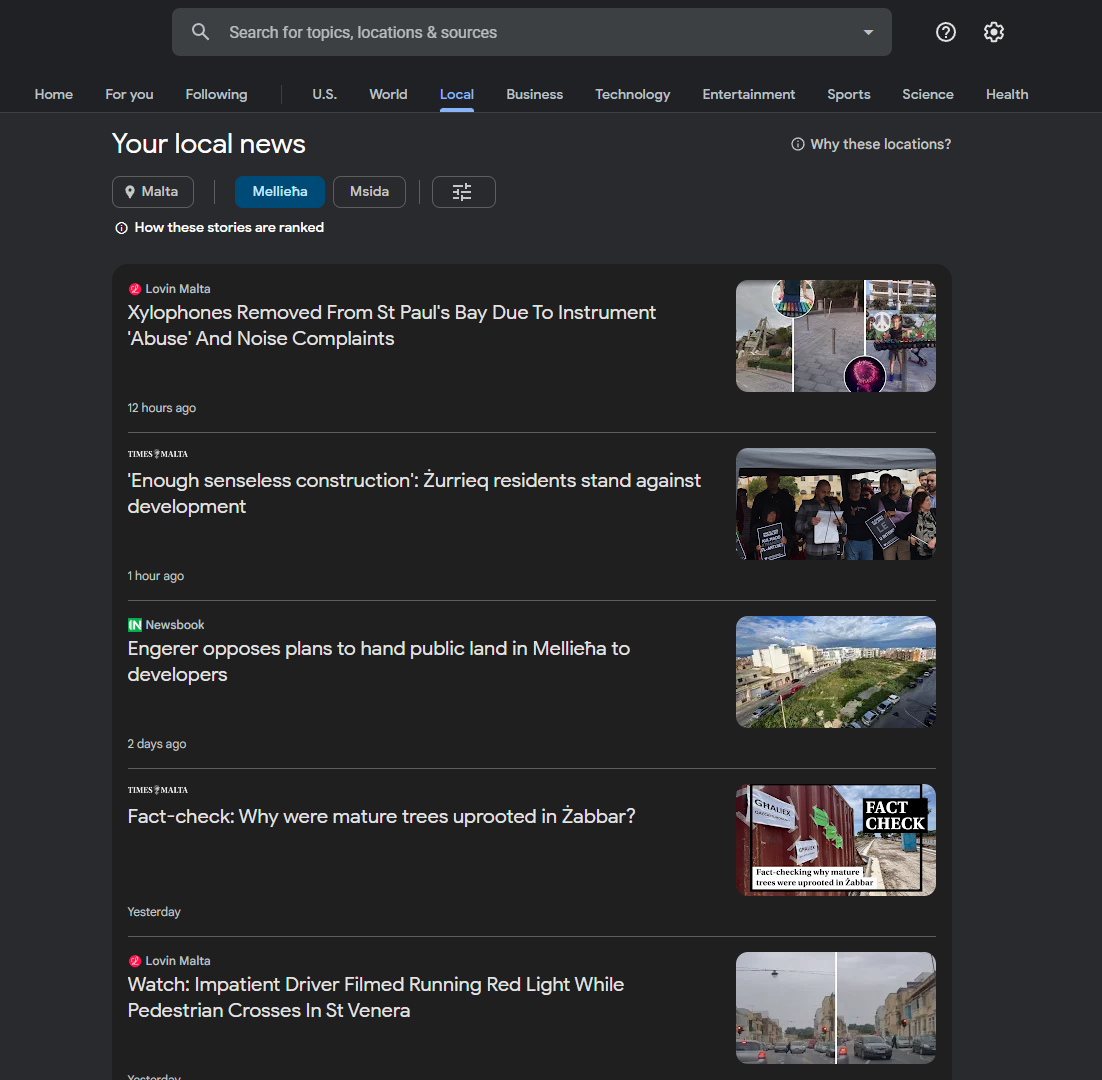
\includegraphics[width=0.5\textwidth]{./figures/googlenewsmellieha.png} \\
    Figure 1: Google News filtering by village (Mellieha) displaying articles which took place in St. Paul's Bay, Żurrieq and Żabbar
  \end{center}
  

  BBC News also offers this feature to a limited extent in its \href{https://www.bbc.com/news/world}{World} section, allowing users to filter news articles on a per-continent basis. However, this feature is not available for smaller geographical regions such as, and as such, cannot tailor news to a user based on the country they live in, let alone the specific city/village.

  
  \section{Methodology}
  \subsection{Dataset}
  \textit{All source files for work related to this section can be found in the} \verb|docs/data| \textit{directory}

  \medskip

  To create a dataset of Maltese news articles, I created an algorithm (found in \verb|scraper.ipynb|) which scrapes news articles in the \href{https://newsbook.com.mt/}{Newsbook} English local archive (found \href{https://newsbook.com.mt/en/category/news/local/}{here}). I was able to scrape the following content of 5797 articles: URL, title, date, and article text. This dataset can be found in \verb|all_articles.csv|. I proceeded to clean this dataset (specifically removing duplicates) in Google Sheets, followed by a filtering process to only include articles which mention the names of Maltese villages (found in \verb|villages.txt|) in their text, as well as the start and end index of these villages within the text (this is required to train the NER model), resulting in a dataset of 2454 articles (found in \verb|location_articles.csv|). The code for this filtering process can be found in \verb|location_extractor.ipynb|. A final pass through of the dataset was carried out to get the URL of each articles' corresponding image (if any) and add it to the dataset (this was also done in \verb|location_extractor.ipynb|), resulting in the final dataset of 2454 articles (found in \verb|location_articles_images.csv|).

  \subsection{Model}
  \textit{All source files for work related to this section can be found in the} \verb|docs/data| \textit{directory}

  \medskip

  The Named Entity Recognition model for this project was trained using the \href{}{spaCy} library in Python. spaCy is an open-source library for NLP written in Python, which provides a wide range of NLP tools and features, including the ability to train custom NER models.
  
  I used the blank English model provided by spaCy as a base model (with the intention of creating a model targetted towards the recognition of the names of Maltese villages), and proceeded to train it on the \verb|location_articles_images| dataset, taking the news article text and corresponding village name indices and entity labels (scraped in the Dataset subsection) as inputs. The model was trained for 10 epochs, with a dropout rate of 0.3.
  
  \begin{center}
    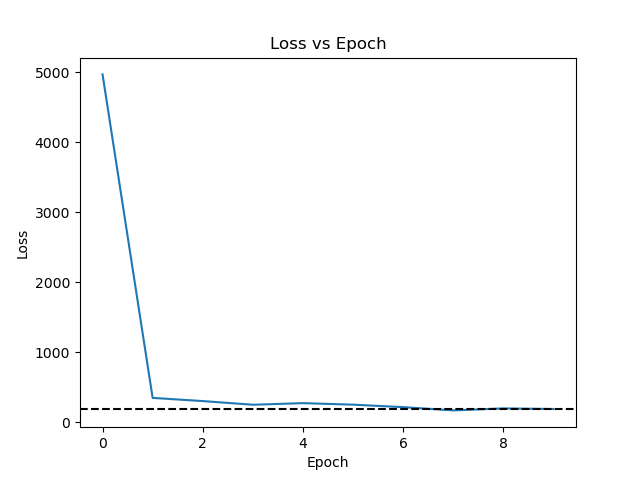
\includegraphics[width=0.5\textwidth]{./figures/nerloss.png} \\
    Figure 2: Loss of the NER model over 10 epochs
  \end{center}

  The code used to train the model can be found in \verb|train_model.ipynb|. The model was saved in the \verb|model| directory.


  \subsection{Web Application}
  \textit{All source files for work related to this section can be found in the} \verb|docs| \textit{directory}
  
  \medskip

  % Overview (mention mobile responsiveness, OpenStreetMap, etc.)
  The web application for this project was developed using PHP, CSS, JavaScript and Python. The application must be hosted (this can be done locally using open-source software such as \href{https://www.apachefriends.org/}{XAMPP}).

  The application is mobile responsive, allowing users to access it from whichever device they prefer.
  
  The application makes use of the \href{https://www.openstreetmap.org/}{OpenStreetMap} API to display a map of Malta on the home page, as well find the coordinates of the villages identified by the Article Location Detector and subsequently display said villages on the map. The Navigator Geolocation API is used on the the News page to ask the user for permission to access their location, which, if provided, is used to automatically filter the news articles in the database based on the village the user is currently in.

  \subsubsection{Home Page} 
  The home page contains a form (called the Article Location Detector) which allows the user to input a news article URL, which is then passed to the NER model to attempt to identify the Maltese village in which the article took place.

  \subsubsection{News Page}
  The news page contains a form (called the Database Lookup) which allows the user to either provide their current location or select a village manually, which is then passed to a python script which filters the \verb|location_articles_images.csv| dataset, and retrieves news articles which took place in that village. Where an article took place is determined by checking which village name occurred most frequently in the article text, and if there is a tie, the village name which occurred first is chosen. The articles are then displayed on a grid of cards, each containing the article title, date, image (if any), and a link to the original article. The cards are sorted by date, with the most recent articles appearing first.

  
  \section{Results}
  \subsection{Dataset}
  % Mention good coverage of all villages but may be biased towards more active ones such as Valletta


  \subsection{Model}
  % Do some testing


  \subsection{Web Application}
  % Show screenshots of the web app
  


  
  \section{Challenges and Limitations}
  % Mention the lack of a Maltese NER model, and the lack of a Maltese NLP library

  % English articles only

  % Village names containing multiple words (e.g. St. Paul's Bay)




  \section{Conclusion}
  \lipsum[1]



  \newpage


  \Urlmuskip=0mu plus 1mu\relax
  \bibliographystyle{IEEEtran}
  \bibliography{refs}

\end{multicols*}


\end{document}